% Figure 15: the motor-assembly line of the published case (Zhao et al. 2026).
%
% Compiled by industrial_case/export.py (schematic) from this directory, so
% the shared preamble is found by its relative path. The page is exactly the
% printed text width (164.6 mm), and the manuscript includes it without a
% scaling key.
%
% What is drawn and where it comes from
%   * Published: four DC motor types of one family (models in the legend), the
%     order of 5/4/4/3 units and a line of five stations in a fixed route.
%   * Reconstruction (Section 6.9): one installed module per station and four
%     product-specific modules per station, twenty in all, mounted by a worker
%     in a triangular fuzzy time.
%   * The line is drawn at one instant of the HCMAGRL schedule with seed 42 at
%     equal weights (Figure 17): S1 processes B, S2 is changed over from A to B,
%     S3 to S5 process A. Module and motor colours are the type colours of
%     Figure 17.
%   * Illustrative: the operation panels (a) to (e) follow the usual assembly
%     sequence of permanent-magnet DC motors. The source reports the processing
%     time of every type at every station but not the station operations, and
%     the caption says so.
\documentclass[border=0pt]{standalone}
% Shared TikZ style contract for every schematic figure in this paper.
% Each schematic is a standalone document that \input's this file, so the
% schematics and the matplotlib data figures form one visual system.
%
% Colours are the same Okabe-Ito values as figures/scifig_style.py.

% No font package: the manuscript class sets the body in Computer Modern, so
% the schematics inherit the same family by loading nothing here.
\usepackage{amsmath,amssymb}
\usepackage{tikz}
\usetikzlibrary{arrows.meta,positioning,calc,fit,backgrounds,shapes.geometric,
                shapes.multipart,patterns,decorations.pathreplacing,matrix}

% ---------- Notation shared with the manuscript ----------
% Kept in sync with the definitions in main.tex so that a symbol means the
% same thing in a schematic as it does in the body.
\newcommand{\Cmax}{C_{\max}}
\newcommand{\Zcost}{Z}
\newcommand{\Nb}{\mathcal{N}}

% ---------- Okabe-Ito colour-blind-safe palette ----------
\definecolor{oiblue}{RGB}{0,114,178}
\definecolor{oiorange}{RGB}{230,159,0}
\definecolor{oigreen}{RGB}{0,158,115}
\definecolor{oivermilion}{RGB}{213,94,0}
\definecolor{oipurple}{RGB}{204,121,167}
\definecolor{oisky}{RGB}{86,180,233}
\definecolor{oiyellow}{RGB}{240,228,66}
\definecolor{oigray}{RGB}{110,110,110}

% ---------- Shared node and arrow styles ----------
\tikzset{
  block/.style={draw, rounded corners=2pt, minimum height=6.5mm, minimum width=17mm,
                align=center, font=\footnotesize, fill=oisky!16, line width=0.6pt,
                draw=oiblue!70},
  keyblock/.style={block, fill=oiorange!26, draw=oiorange!85},
  smallblock/.style={block, minimum height=5mm, minimum width=12mm, font=\scriptsize},
  datanode/.style={draw, trapezium, trapezium left angle=70, trapezium right angle=110,
                   align=center, font=\scriptsize, fill=oigreen!14, line width=0.6pt,
                   draw=oigreen!75, inner sep=2pt},
  opnode/.style={draw, circle, inner sep=1pt, minimum size=6mm, font=\scriptsize,
                 fill=oiyellow!45, line width=0.6pt, draw=oigray},
  macnode/.style={draw, rectangle, rounded corners=1pt, minimum size=6mm,
                  font=\scriptsize, fill=oisky!30, line width=0.6pt, draw=oiblue!70},
  modnode/.style={draw, diamond, aspect=1.4, inner sep=1pt, minimum size=6mm,
                  font=\scriptsize, fill=oipurple!28, line width=0.6pt, draw=oipurple!85},
  arrow/.style={-{Stealth[length=2.0mm]}, line width=0.65pt},
  dasharrow/.style={arrow, dashed, draw=oigray},
  thinedge/.style={line width=0.45pt, draw=oigray},
  note/.style={font=\scriptsize, text=oigray, align=center},
  tinynote/.style={font=\tiny, text=oigray, align=center},
  group/.style={draw=oigray, dashed, rounded corners=3pt, inner sep=2.6mm,
                line width=0.5pt},
  grouplabel/.style={font=\scriptsize\itshape, text=oigray},
  whitebg/.style={fill=white, inner sep=1pt},
}

% ---------- materials ----------
\definecolor{steel}{RGB}{160,168,178}
\definecolor{steeldk}{RGB}{86,94,106}
\definecolor{steellt}{RGB}{236,239,242}
\definecolor{copper}{RGB}{190,112,50}
\definecolor{copperdk}{RGB}{118,64,22}
\definecolor{copperlt}{RGB}{240,186,128}
\definecolor{framec}{RGB}{58,70,84}
\definecolor{framelt}{RGB}{122,136,152}
\definecolor{ferrite}{RGB}{66,68,74}
\definecolor{skin}{RGB}{238,196,150}
\definecolor{plastic}{RGB}{44,48,54}
\colorlet{tA}{oiblue}\colorlet{tB}{oiorange}\colorlet{tC}{oigreen}\colorlet{tD}{oipurple}
\tikzset{
  cyl/.style={left color=steeldk, right color=steeldk, middle color=steellt},
  hcyl/.style={top color=steeldk, bottom color=steeldk, middle color=steellt},
  motion/.style={-{Stealth[length=1.5mm,width=1.3mm]}, draw=oivermilion, line width=0.8pt},
  panel/.style={rounded corners=1.4mm, top color=white, bottom color=steellt!70},
  oplabel/.style={font=\scriptsize, text=framec, anchor=base},
  plabel/.style={font=\scriptsize\bfseries, text=framec, anchor=north west, inner sep=0},
}
% Vertical datum of the line: floor line, belt top, beam top.
\def\yF{31}\def\yB{38.5}\def\yT{58.8}
% upright motor: base centre (#1,#2), half width #3, body height #4, type colour #5
\newcommand{\motor}[5]{%
  \shade[cyl, draw=steeldk, line width=0.2pt] ({#1-#3},#2) rectangle ({#1+#3},{#2+#4});
  \shade[left color=#5!65!black, right color=#5!65!black, middle color=#5!60!white]
    ({#1-#3},{#2+0.36*#4}) rectangle ({#1+#3},{#2+0.66*#4});
  \fill[steel, draw=steeldk, line width=0.2pt] (#1,{#2+#4}) ellipse ({#3} and {0.3*#3});
  \fill[steeldk!55] (#1,{#2+#4}) ellipse ({0.42*#3} and {0.13*#3});
  \shade[cyl] ({#1-0.13*#3},{#2+#4}) rectangle ({#1+0.13*#3},{#2+#4+1.0});}
% motor on its pallet on the belt: x, half width, height, colour
\newcommand{\onpallet}[4]{%
  \fill[framec, rounded corners=0.3mm] ({#1-#2-0.8},\yB) rectangle ({#1+#2+0.8},{\yB+1.3});
  \fill[framelt] ({#1-#2-0.5},{\yB+1.0}) rectangle ({#1+#2+0.5},{\yB+1.3});
  \motor{#1}{\yB+1.3}{#2}{#3}{#4}}
% product-specific module: centre x #1, bottom #2, colour #3, letter #4
\newcommand{\module}[4]{%
  \fill[#3!70!black, rounded corners=0.35mm] ({#1-2.15},#2) rectangle ({#1+2.15},{#2+3.8});
  \shade[top color=#3!72!white, bottom color=#3, rounded corners=0.25mm]
    ({#1-1.95},{#2+0.2}) rectangle ({#1+1.95},{#2+3.3});
  \fill[steeldk] ({#1-1.45},{#2+3.8}) rectangle ({#1-0.95},{#2+4.35});
  \fill[steeldk] ({#1+0.95},{#2+3.8}) rectangle ({#1+1.45},{#2+4.35});
  \node[font=\scriptsize\bfseries, text=white, inner sep=0] at (#1,{#2+1.75}) {#4};}
\newcommand{\emptyslot}[3]{% x, bottom, colour
  \draw[#3, dashed, line width=0.4pt, rounded corners=0.35mm]
    ({#1-2.15},#2) rectangle ({#1+2.15},{#2+3.8});}
% tool cart holding the four modules of one station
\newcommand{\cart}[1]{%
  \shade[top color=gray!14, bottom color=gray!36, rounded corners=0.4mm]
    ({#1-9.7},11.4) rectangle ({#1+9.7},17.4);
  \draw[framelt, line width=0.3pt, rounded corners=0.4mm] ({#1-9.7},11.4) rectangle ({#1+9.7},17.4);
  \draw[framelt, line width=0.3pt] ({#1-9.7},14.4) -- ({#1+9.7},14.4);
  \fill[framelt] ({#1-1.6},15.7) rectangle ({#1+1.6},16.1);
  \fill[framelt] ({#1-1.6},12.7) rectangle ({#1+1.6},13.1);
  \fill[framec, rounded corners=0.2mm] ({#1-10.2},17.4) rectangle ({#1+10.2},18.2);
  \draw[framec, line width=0.9pt, line cap=round] ({#1-10.2},17.9) -- ({#1-11.4},20.8);
  \foreach \dx in {-7.4,7.4} {\fill[black!78] ({#1+\dx},10.4) circle (1.05);
                               \fill[gray!45] ({#1+\dx},10.4) circle (0.38);}}
% station frame over the belt: centre #1, label #2, lit status lamp #3 (0 green, 1 amber)
\newcommand{\station}[3]{%
  \fill[framec] ({#1-10.5},\yF) rectangle ({#1-9.3},{\yT-2.3});
  \fill[framec] ({#1+9.3},\yF) rectangle ({#1+10.5},{\yT-2.3});
  \fill[framelt!55] ({#1-10.3},\yF) rectangle ({#1-10.0},{\yT-2.3});
  \fill[framelt!55] ({#1+9.5},\yF) rectangle ({#1+9.8},{\yT-2.3});
  \shade[top color=framelt, bottom color=framec, rounded corners=0.3mm]
    ({#1-11.2},{\yT-3.1}) rectangle ({#1+11.2},\yT);
  \node[fill=white, rounded corners=0.5mm, inner sep=0.5mm, font=\scriptsize\bfseries,
        text=framec] at (#1,{\yT-1.55}) {#2};
  \shade[cyl] ({#1-1.4},{\yT-4.9}) rectangle ({#1+1.4},{\yT-3.1});
  \fill[framec, rounded corners=0.2mm] ({#1-4.6},{\yT-5.9}) rectangle ({#1+4.6},{\yT-4.9});
  % status lamp
  \fill[framec] ({#1+7.6},\yT) rectangle ({#1+7.95},{\yT+0.8});
  \foreach \k/\c in {0/oigreen, 1/oiorange, 2/oivermilion} {
    \ifnum\k=#3 \fill[\c] ({#1+7.05},{\yT+0.8+1.05*\k}) rectangle ({#1+8.5},{\yT+1.75+1.05*\k});
    \else \fill[\c!22!white] ({#1+7.05},{\yT+0.8+1.05*\k}) rectangle ({#1+8.5},{\yT+1.75+1.05*\k}); \fi}
  \fill[framec] ({#1+7.05},{\yT+3.95}) rectangle ({#1+8.5},{\yT+4.25});}
% installed module with its tool tip: centre, colour, letter
\newcommand{\toolhead}[3]{%
  \fill[steeldk] ({#1-1.2},{\yT-9.7}) -- ({#1+1.2},{\yT-9.7}) -- ({#1+0.6},{\yT-11.2}) -- ({#1-0.6},{\yT-11.2}) -- cycle;
  \module{#1}{\yT-9.7}{#2}{#3}}
\begin{document}
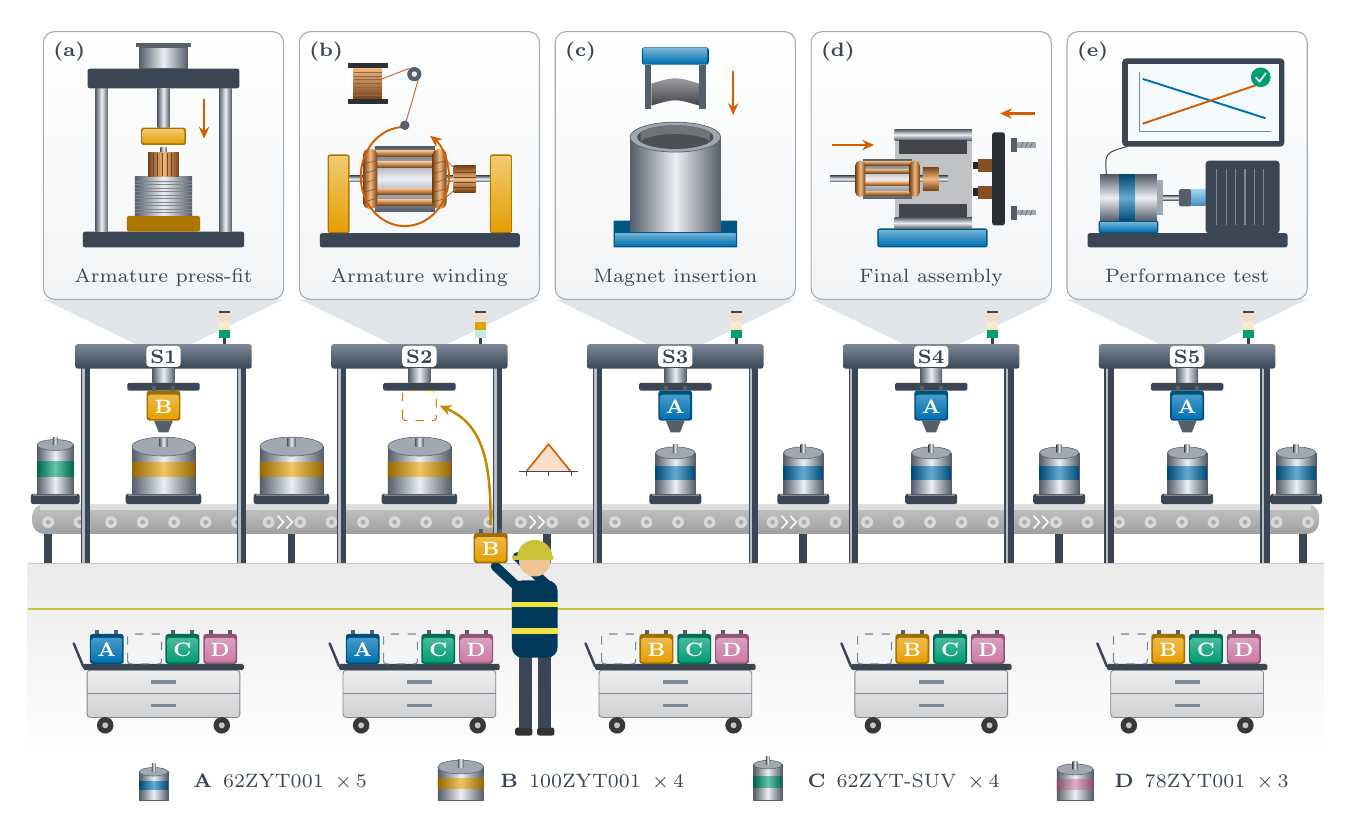
\begin{tikzpicture}[x=1mm, y=1mm, line join=round]
\useasboundingbox (0,0) rectangle (164.6,99);

% =====================================================================
% Operation panels and the zoom from each station
% =====================================================================
\def\pY{64.5}
\foreach \i/\x in {0/17.25,1/49.75,2/82.25,3/114.75,4/147.25} {
  \pgfmathsetmacro{\xa}{2+32.5*\i}
  \pgfmathsetmacro{\xb}{\xa+30.5}
  \fill[framelt!22] ({\x-3.5},\yT) -- ({\x+3.5},\yT) -- (\xb,\pY) -- (\xa,\pY) -- cycle;
  \shade[panel] (\xa,\pY) rectangle (\xb,{\pY+34});
  \draw[framelt!70, line width=0.4pt, rounded corners=1.4mm] (\xa,\pY) rectangle (\xb,{\pY+34});
}

% =====================================================================
% Line view
% =====================================================================
\shade[top color=gray!16, bottom color=white] (0,7) rectangle (164.6,\yF);
\draw[gray!45, line width=0.3pt] (0,\yF) -- (164.6,\yF);
\draw[oiyellow!85!black, line width=0.7pt] (0,25.2) -- (164.6,25.2);

% conveyor
\foreach \x in {2.6,33.5,66,98.5,131,162} {
  \fill[framec] ({\x-0.5},\yF) rectangle ({\x+0.5},{\yB-3.6});}
\shade[top color=gray!45, bottom color=gray!75, rounded corners=1.5mm] (0.6,{\yB-3.8}) rectangle (164,\yB);
\fill[gray!25] (1.6,{\yB-0.7}) rectangle (163,\yB);
\foreach \x in {2.6,6.6,...,162.6} {\fill[gray!30] (\x,{\yB-2.3}) circle (0.75);
                                     \fill[gray!65] (\x,{\yB-2.3}) circle (0.3);}
% flow direction, centred between two rollers in each gap
\foreach \x in {31.75,63.75,95.75,127.75} {
  \foreach \d in {0,1.1} {\draw[white, line width=0.55pt] ({\x+\d},{\yB-1.5}) -- ({\x+\d+0.75},{\yB-2.3}) -- ({\x+\d},{\yB-3.1});}}

% stations, installed modules (S2 is being changed over to B)
\foreach \x/\s/\l in {17.25/S1/0, 49.75/S2/1, 82.25/S3/0, 114.75/S4/0, 147.25/S5/0} {\station{\x}{\s}{\l}}
\toolhead{17.25}{tB}{B}
\toolhead{82.25}{tA}{A}
\toolhead{114.75}{tA}{A}
\toolhead{147.25}{tA}{A}
\emptyslot{49.75}{\yT-9.7}{tB!85!black}

% motors on pallets, a snapshot of the schedule
\onpallet{3.5}{2.3}{6.2}{tC}
\onpallet{17.25}{4.0}{6.0}{tB}
\onpallet{33.5}{4.0}{6.0}{tB}
\onpallet{49.75}{4.0}{6.0}{tB}
\onpallet{82.25}{2.5}{5.2}{tA}
\onpallet{98.5}{2.5}{5.2}{tA}
\onpallet{114.75}{2.5}{5.2}{tA}
\onpallet{131}{2.5}{5.2}{tA}
\onpallet{147.25}{2.5}{5.2}{tA}
\onpallet{161.1}{2.5}{5.2}{tA}

% tool carts with the twenty product-specific modules
\foreach \x in {17.25,49.75,82.25,114.75,147.25} {\cart{\x}}
\module{10.05}{18.2}{tA}{A}\emptyslot{14.85}{18.2}{framelt}\module{19.65}{18.2}{tC}{C}\module{24.45}{18.2}{tD}{D}
\module{42.55}{18.2}{tA}{A}\emptyslot{47.35}{18.2}{framelt}\module{52.15}{18.2}{tC}{C}\module{56.95}{18.2}{tD}{D}
\foreach \x in {82.25,114.75,147.25} {
  \emptyslot{\x-7.2}{18.2}{framelt}\module{\x-2.4}{18.2}{tB}{B}\module{\x+2.4}{18.2}{tC}{C}\module{\x+7.2}{18.2}{tD}{D}}

% worker mounting module B on S2
\begin{scope}[shift={(64.4,9.4)}]
  \fill[black!80, rounded corners=0.3mm] (-2.5,-0.3) rectangle (-0.3,0.7);
  \fill[black!80, rounded corners=0.3mm] (0.3,-0.3) rectangle (2.5,0.7);
  \fill[framec] (-2.0,0.6) rectangle (-0.35,10.2);
  \fill[framec] (0.35,0.6) rectangle (2.0,10.2);
  \fill[oiblue!50!black, rounded corners=1.3mm] (-2.9,9.6) rectangle (2.9,19.4);
  \fill[oiyellow] (-2.9,12.6) rectangle (2.9,13.3);
  \fill[oiyellow] (-2.9,16.0) rectangle (2.9,16.7);
  \draw[oiblue!50!black, line width=3.4pt, line cap=round] (-2.0,18.4) -- (-5.0,21.2);
  \draw[oiblue!50!black, line width=3.4pt, line cap=round] (2.0,18.4) -- (-2.2,22.4);
  \fill[skin] (0,21.9) circle (2.0);
  \fill[oiyellow!85!black] (-2.25,22.3) arc (180:0:2.25) -- cycle;
  \fill[oiyellow!85!black, rounded corners=0.2mm] (-2.9,22.0) rectangle (2.4,22.55);
\end{scope}
\module{58.8}{31.0}{tB}{B}
\draw[motion, draw=tB!85!black, line width=0.9pt] (58.8,35.8) .. controls (58.8,43) and (58.2,48.5) .. (52.3,51.0);
% the mount takes a worker-dependent triangular fuzzy time
\begin{scope}[shift={(62.4,42.6)}]
  \fill[oivermilion!20] (0.9,0) -- (3.75,3.5) -- (6.6,0) -- cycle;
  \draw[oivermilion, line width=0.6pt] (0.9,0) -- (3.75,3.5) -- (6.6,0);
  \draw[framec, line width=0.35pt] (0,0) -- (7.5,0);
  \foreach \t in {0.9,3.75,6.6} \draw[framec, line width=0.35pt] (\t,0) -- (\t,-0.6);
\end{scope}

% (a) armature press-fit ------------------------------------------------
\begin{scope}[shift={(2,\pY)}]
  \node[plabel] at (1.2,32.8) {(a)};
  \fill[framec, rounded corners=0.3mm] (5,6.6) rectangle (25.5,8.6);
  \shade[cyl] (6.6,8.6) rectangle (8.2,26.8);
  \shade[cyl] (22.3,8.6) rectangle (23.9,26.8);
  \fill[framec, rounded corners=0.3mm] (5.6,26.8) rectangle (24.9,29.3);
  \shade[cyl, draw=steeldk, line width=0.2pt] (12.2,29.3) rectangle (18.3,32.0);
  \fill[steeldk] (11.8,32.0) rectangle (18.7,32.6);
  \shade[cyl] (14.5,21.8) rectangle (16.0,26.8);
  \fill[tB!75!black, rounded corners=0.3mm] (12.4,19.6) rectangle (18.1,21.8);
  \shade[top color=tB!55!white, bottom color=tB, rounded corners=0.2mm] (12.6,19.8) rectangle (17.9,21.6);
  \fill[tB!75!black, rounded corners=0.3mm] (10.6,8.6) rectangle (19.9,10.6);
  \shade[cyl] (14.85,10.6) rectangle (15.65,19.3);
  \shade[cyl] (11.6,10.6) rectangle (18.9,15.6);
  \foreach \yy in {11.0,11.45,...,15.4} \draw[steeldk!75, line width=0.15pt] (11.6,\yy) -- (18.9,\yy);
  \shade[left color=copperdk, right color=copperdk, middle color=copperlt] (13.3,15.6) rectangle (17.2,18.6);
  \foreach \xx in {13.9,14.5,...,16.8} \draw[copperdk, line width=0.2pt] (\xx,15.6) -- (\xx,18.6);
  \draw[motion] (20.4,25.4) -- (20.4,20.4);
  \node[oplabel] at (15.25,2.2) {Armature press-fit};
\end{scope}

% (b) armature winding --------------------------------------------------
\begin{scope}[shift={(34.5,\pY)}]
  \node[plabel] at (1.2,32.8) {(b)};
  \fill[framec, rounded corners=0.3mm] (2.6,6.6) rectangle (28,8.4);
  \fill[tB!75!black, rounded corners=0.3mm] (3.6,8.4) rectangle (6.4,18.4);
  \fill[tB!75!black, rounded corners=0.3mm] (24.2,8.4) rectangle (27.0,18.4);
  \shade[top color=tB!55!white, bottom color=tB] (3.8,8.6) rectangle (6.2,18.2);
  \shade[top color=tB!55!white, bottom color=tB] (24.4,8.6) rectangle (26.8,18.2);
  \shade[hcyl] (6.4,14.9) rectangle (24.2,15.7);
  \shade[hcyl] (9.6,11.2) rectangle (17.2,19.4);
  \foreach \yy in {11.9,13.3,16.7,18.1} {
    \shade[top color=copperlt, bottom color=copperdk] (9.6,\yy) rectangle (17.2,{\yy+0.75});}
  \shade[left color=copperdk, right color=copperdk, middle color=copperlt, rounded corners=0.7mm] (8.1,11.5) rectangle (9.9,19.1);
  \shade[left color=copperdk, right color=copperdk, middle color=copperlt, rounded corners=0.7mm] (16.9,11.5) rectangle (18.7,19.1);
  \foreach \yy in {12.4,13.6,...,18.4} {
    \draw[copperdk, line width=0.15pt] (8.3,\yy) -- (9.7,{\yy+0.4});
    \draw[copperdk, line width=0.15pt] (17.1,\yy) -- (18.5,{\yy+0.4});}
  \shade[top color=copperdk, bottom color=copperdk, middle color=copperlt] (19.6,13.6) rectangle (22.4,17.0);
  \foreach \yy in {14.2,14.85,...,16.6} \draw[copperdk, line width=0.2pt] (19.6,\yy) -- (22.4,\yy);
  \draw[copper, line width=0.35pt] (18.7,17.6) -- (19.8,16.6);
  \draw[copper, line width=0.35pt] (18.7,13.0) -- (19.8,14.0);
  \draw[motion, line width=0.7pt] (13.4,21.9) arc (90:415:5.6 and 6.3);
  \shade[top color=copperlt, bottom color=copperdk] (6.9,25.4) rectangle (10.5,29.4);
  \foreach \yy in {25.9,26.4,...,29.0} \draw[copperdk!80, line width=0.12pt] (6.9,\yy) -- (10.5,\yy);
  \fill[plastic] (6.2,24.8) rectangle (11.2,25.4);
  \fill[plastic] (6.2,29.4) rectangle (11.2,30.0);
  \fill[steeldk] (14.6,28.6) circle (0.9);
  \fill[steellt] (14.6,28.6) circle (0.35);
  \draw[copper, line width=0.35pt] (10.5,28.0) -- (13.9,29.3);
  \draw[copper, line width=0.35pt] (15.1,27.9) .. controls (14.4,25.4) .. (13.5,22.4);
  \fill[steeldk] (13.4,22.1) circle (0.6);
  \node[oplabel] at (15.25,2.2) {Armature winding};
\end{scope}

% (c) magnet insertion --------------------------------------------------
\begin{scope}[shift={(67,\pY)}]
  \node[plabel] at (1.2,32.8) {(c)};
  \fill[tA!75!black] (7.4,6.6) -- (23.1,6.6) -- (23.1,10.0) -- (21.0,10.0) -- (21.0,8.6) -- (9.5,8.6) -- (9.5,10.0) -- (7.4,10.0) -- cycle;
  \shade[top color=tA!55!white, bottom color=tA] (7.6,6.8) rectangle (22.9,8.4);
  \shade[cyl] (9.5,8.6) rectangle (21.0,20.6);
  \fill[steel, draw=steeldk, line width=0.25pt] (15.25,20.6) ellipse (5.75 and 1.9);
  \fill[plastic!85] (15.25,20.6) ellipse (4.85 and 1.5);
  \fill[ferrite!75!white] ($(15.25,20.6)+(25:4.85 and 1.5)$) arc (25:155:4.85 and 1.5)
       -- ++(0,-1.1) arc (155:25:4.85 and 1.5) -- cycle;
  \shade[top color=ferrite!50!white, bottom color=ferrite]
    (12.2,24.6) .. controls (15.25,25.5) .. (18.3,24.6) -- (18.3,27.4) .. controls (15.25,28.3) .. (12.2,27.4) -- cycle;
  \fill[tA!75!black, rounded corners=0.3mm] (11.0,29.8) rectangle (19.5,32.0);
  \shade[top color=tA!55!white, bottom color=tA] (11.2,30.0) rectangle (19.3,31.8);
  \fill[steeldk] (11.4,24.2) rectangle (12.2,29.8);
  \fill[steeldk] (18.3,24.2) rectangle (19.1,29.8);
  \draw[motion] (22.6,29.0) -- (22.6,23.4);
  \node[oplabel] at (15.25,2.2) {Magnet insertion};
\end{scope}

% (d) final assembly ----------------------------------------------------
\begin{scope}[shift={(99.5,\pY)}]
  \node[plabel] at (1.2,32.8) {(d)};
  \fill[tA!75!black, rounded corners=0.3mm] (8.4,6.6) rectangle (22.4,9.0);
  \shade[top color=tA!55!white, bottom color=tA] (8.6,6.8) rectangle (22.2,8.8);
  \fill[steellt!60!gray] (10.6,10.4) rectangle (20.4,20.2);
  \shade[hcyl] (10.6,20.2) rectangle (20.4,21.6);
  \shade[hcyl] (10.6,9.0) rectangle (20.4,10.4);
  \fill[ferrite] (11.2,18.5) rectangle (19.8,20.2);
  \fill[ferrite] (11.2,10.4) rectangle (19.8,12.1);
  \shade[hcyl] (2.4,14.9) rectangle (17.4,15.7);
  \shade[hcyl] (6.6,12.8) rectangle (12.8,17.8);
  \foreach \yy in {13.2,14.4,16.0,17.0} {
    \shade[top color=copperlt, bottom color=copperdk] (6.6,\yy) rectangle (12.8,{\yy+0.55});}
  \shade[left color=copperdk, right color=copperdk, middle color=copperlt, rounded corners=0.6mm] (5.6,13.0) rectangle (6.9,17.6);
  \shade[left color=copperdk, right color=copperdk, middle color=copperlt, rounded corners=0.6mm] (12.5,13.0) rectangle (13.8,17.6);
  \shade[top color=copperdk, bottom color=copperdk, middle color=copperlt] (14.2,13.8) rectangle (16.2,16.8);
  \fill[plastic, rounded corners=0.3mm] (23.0,9.4) rectangle (24.6,21.2);
  \fill[copper!70!black] (21.2,16.2) rectangle (23.0,17.8);
  \fill[copper!70!black] (21.2,12.8) rectangle (23.0,14.4);
  \fill[black!85] (20.6,16.5) rectangle (21.2,17.5);
  \fill[black!85] (20.6,13.1) rectangle (21.2,14.1);
  \foreach \yy in {11.0,19.6} {
    \fill[steeldk] (25.4,{\yy-0.9}) rectangle (26.2,{\yy+0.9});
    \fill[steel] (26.2,{\yy-0.35}) rectangle (28.6,{\yy+0.35});
    \foreach \xx in {26.6,27.2,27.8} \draw[steeldk, line width=0.15pt] (\xx,{\yy-0.35}) -- ({\xx+0.3},{\yy+0.35});}
  \draw[motion] (2.6,19.6) -- (8.0,19.6);
  \draw[motion] (28.4,23.6) -- (24.0,23.6);
  \node[oplabel] at (15.25,2.2) {Final assembly};
\end{scope}

% (e) performance test --------------------------------------------------
\begin{scope}[shift={(132,\pY)}]
  \node[plabel] at (1.2,32.8) {(e)};
  \fill[framec, rounded corners=0.3mm] (2.6,6.6) rectangle (28,8.4);
  \fill[tA!75!black, rounded corners=0.3mm] (4.0,8.4) rectangle (11.6,10.0);
  \shade[top color=tA!55!white, bottom color=tA] (4.2,8.6) rectangle (11.4,9.8);
  \shade[hcyl] (4.2,10.0) rectangle (11.4,15.8);
  \shade[top color=tA!65!black, bottom color=tA!65!black, middle color=tA!60!white] (6.6,10.0) rectangle (8.6,15.8);
  \fill[steel] (11.4,10.7) rectangle (12.2,15.1);
  \shade[hcyl] (12.2,12.6) rectangle (14.2,13.2);
  \fill[steeldk, rounded corners=0.2mm] (14.2,11.8) rectangle (15.8,14.0);
  \shade[top color=oisky!60!white, bottom color=oisky!80!black] (15.8,11.9) rectangle (17.6,13.9);
  \fill[framec, rounded corners=0.4mm] (17.6,8.4) rectangle (27.0,17.6);
  \foreach \xx in {19.0,20.2,...,26} \draw[framelt, line width=0.4pt] (\xx,9.4) -- (\xx,16.6);
  \fill[framec, rounded corners=0.5mm] (7.0,19.4) rectangle (27.6,30.6);
  \fill[white!94!oisky] (7.7,20.1) rectangle (26.9,29.9);
  \draw[framelt, line width=0.3pt] (9.2,21.3) -- (9.2,28.9) (9.2,21.3) -- (25.9,21.3);
  \draw[oiblue, line width=0.7pt] (9.6,28.0) -- (25.2,23.0);
  \draw[oivermilion, line width=0.7pt] (9.6,22.3) -- (25.2,27.6);
  \fill[oigreen] (24.6,28.2) circle (1.25);
  \draw[white, line width=0.6pt] (23.95,28.2) -- (24.45,27.65) -- (25.25,28.75);
  \draw[black!75, line width=0.35pt] (5.0,15.8) .. controls (4.8,18.6) .. (7.6,19.4);
  \node[oplabel] at (15.25,2.2) {Performance test};
\end{scope}

% =====================================================================
% Product legend: type, model and quantity of the order
% =====================================================================
\foreach \x/\c/\t/\m/\w/\h/\q in {
    16/tA/A/62ZYT001/1.8/3.6/5, 55/tB/B/100ZYT001/2.9/4.2/4,
    94/tC/C/62ZYT-SUV/1.8/4.5/4, 133/tD/D/78ZYT001/2.3/3.9/3} {
  \motor{\x}{0.9}{\w}{\h}{\c}
  \node[font=\scriptsize, anchor=west, text=framec] at ({\x+3.8},3.2)
    {\textbf{\t}\enspace \m\enspace$\times\,\q$};
}
\end{tikzpicture}
\end{document}
